\documentclass{article}

\usepackage{graphicx}
\usepackage{tikz}
\usepackage{tikzsymbols}
\usetikzlibrary{calc,patterns,shapes.geometric}
\pagestyle{empty}
\usepackage[margin=0pt]{geometry}
\geometry{papersize={14in,12in}}

\def\centerarc[#1](#2)(#3:#4:#5){\draw[#1] ($(#2)+({#5*cos(#3)},{#5*sin(#3)})$) arc (#3:#4:#5);}

\begin{document}
	\begin{figure}
		\centering
		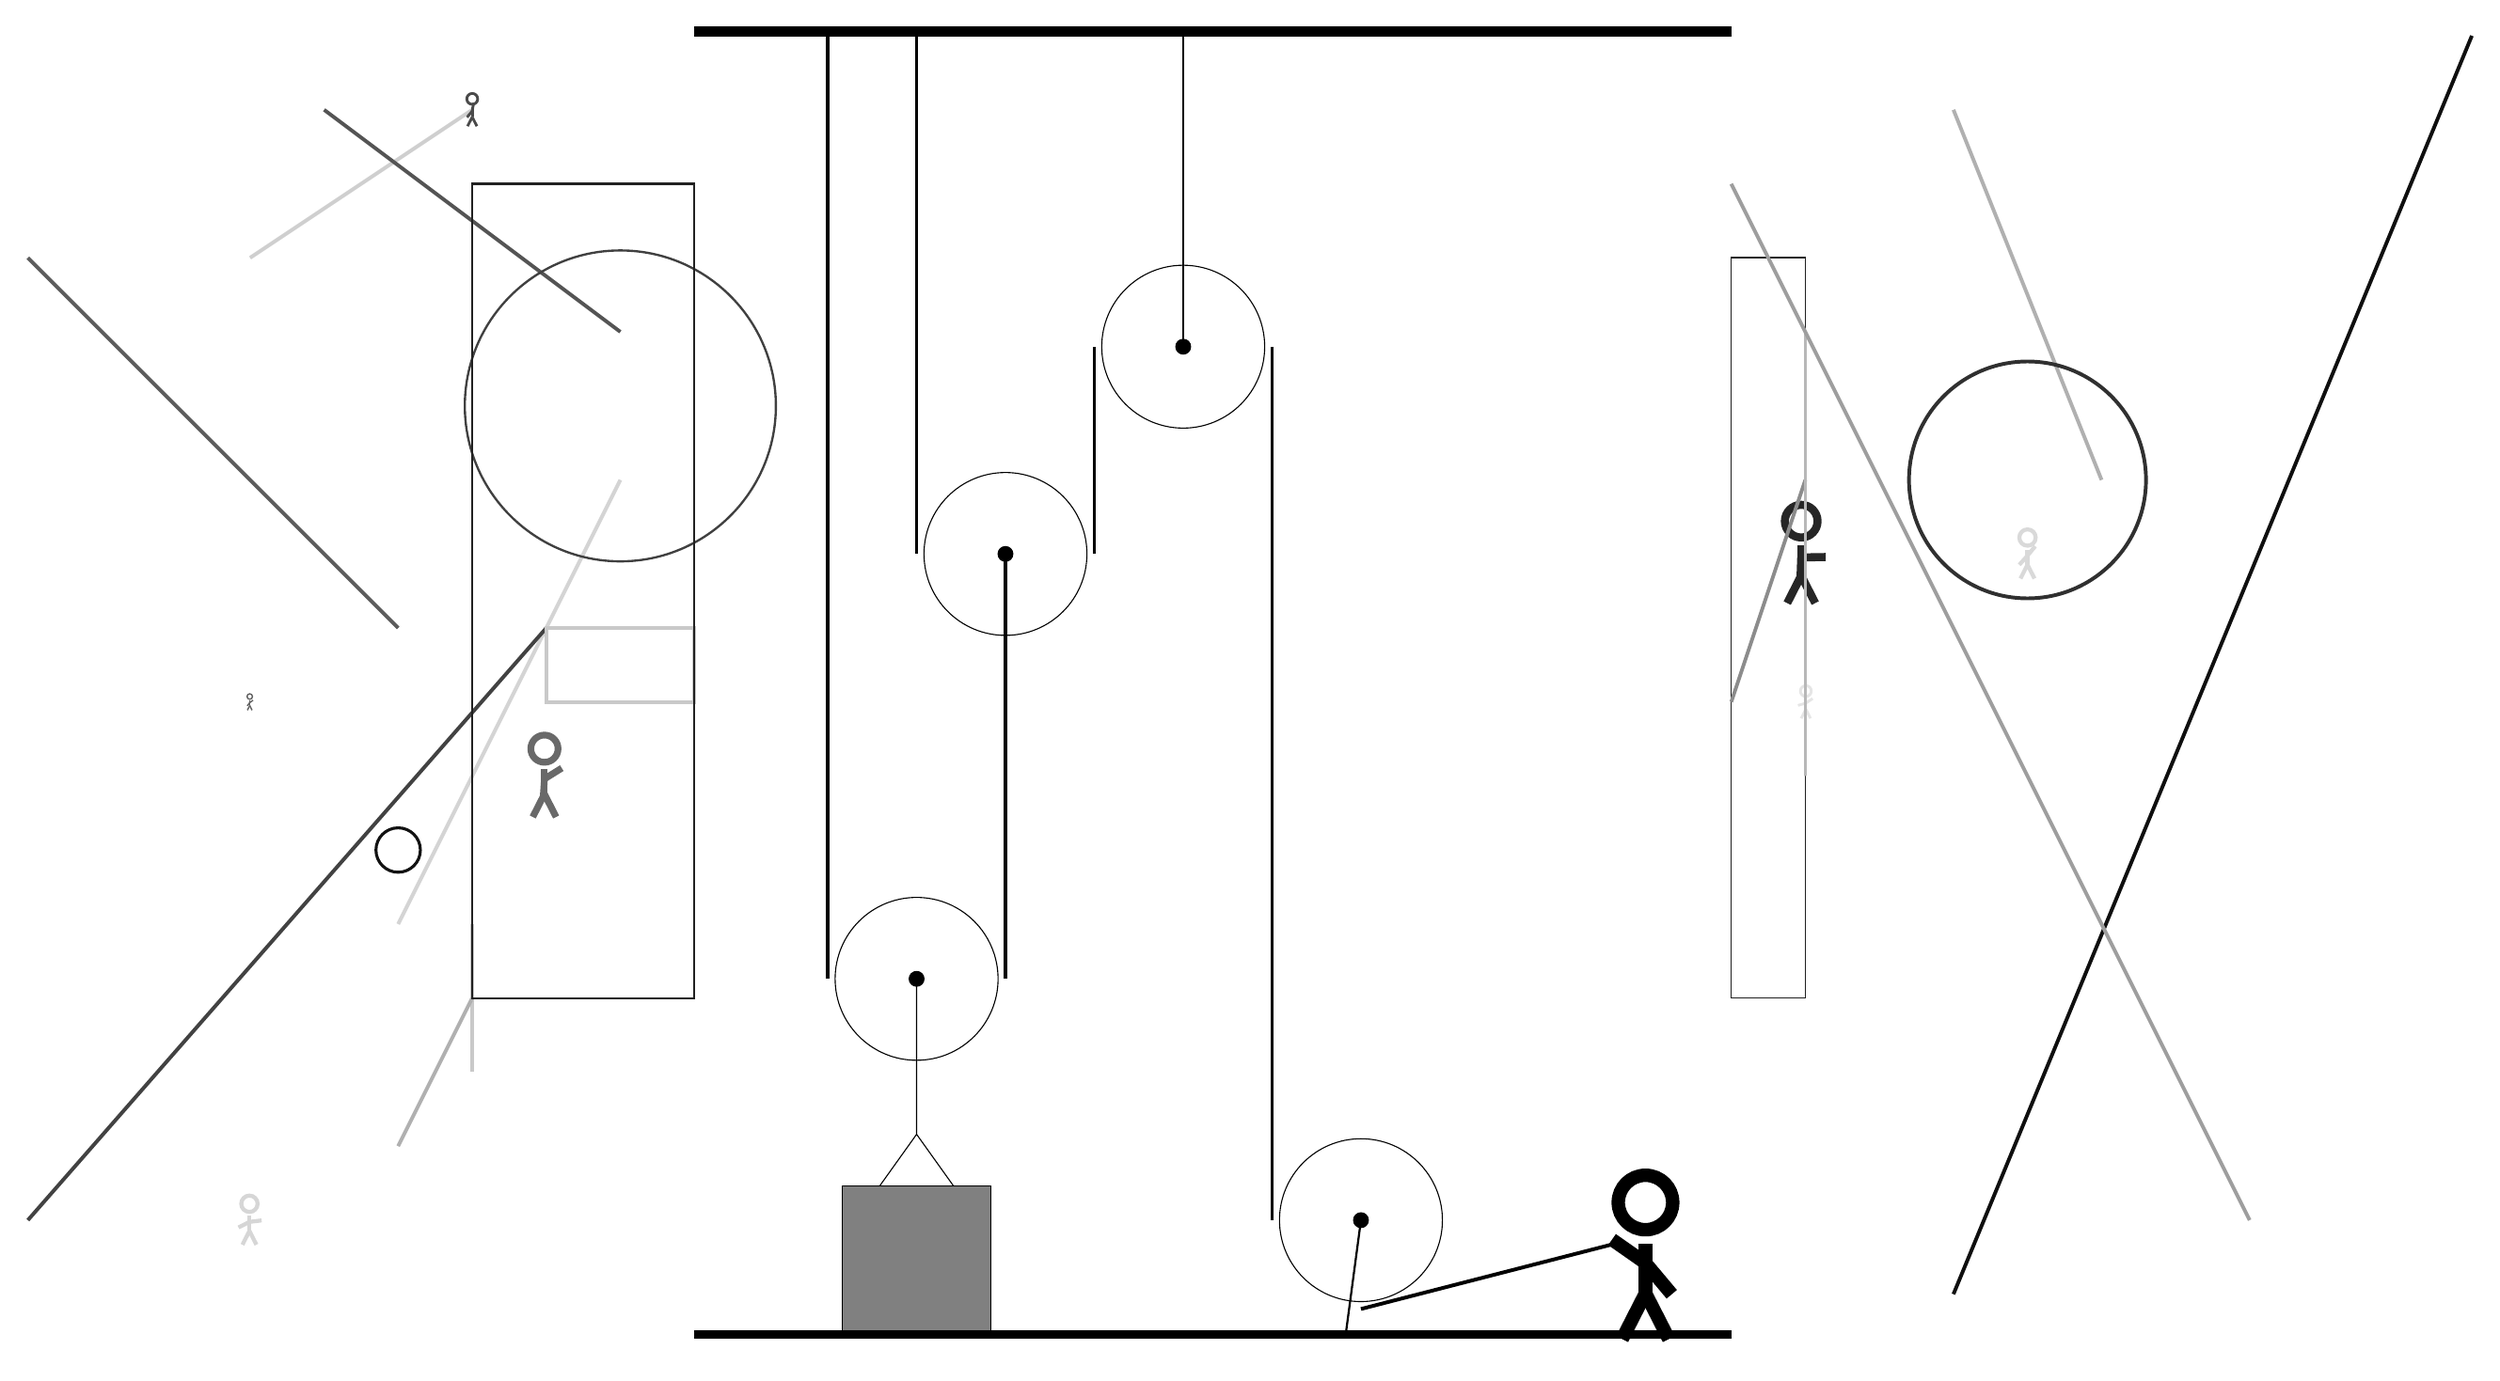
\begin{tikzpicture}
			%%%%% START %%%%%
			
			\draw[fill=black] (-2, 14) rectangle (12, 14.125);
			
			\draw (1, 1.26) circle (1.1);
			\draw[fill=black] (1, 1.26) circle (0.1);
			
			\draw[line width=0.5mm, color=black!21](-5, 0) -- (-5, 2);
			
			\draw[line width=0.5mm, color=black!19](-5, 13) -- (-8, 11);
			\draw[line width=0.5mm, color=black!67](-7, 13) -- (-3, 10);
			\draw [line width=0.4mm, color=black!93](-6, 3) circle (0.3);
			\node[line width=0.6mm, color=black!59] at (-4, 4) {\Strichmaxerl[5][86][32]};
			\node[line width=0.4mm, color=black!85] at (13, 7) {\Strichmaxerl[6][88][1]};
			\draw[line width=0.5mm, color=black!31](15, 13) -- (17, 8);
			\draw[line width=0.2mm, color=black!88] (12, 11) rectangle (13, 1);
			\draw[line width=0.5mm, color=black!64](-6, 6) -- (-11, 11);
			
			\draw[line width=0.5mm, color=black!17](-3, 8) -- (-6, 2);
			\node[line width=0.6mm, color=black!16] at (-8, -2) {\Strichmaxerl[3][27][7]};
			
			\draw[line width=0.5mm, color=black!31](-5, 1) -- (-6, -1);
			\draw [line width=0.3mm, color=black!75](-3, 9) circle (2.1);
			
			\node[line width=0.4mm, color=black!62] at (-8, 5) {\Strichmaxerl[1][53][35]};
			\draw[line width=0.5mm, color=black!74](-4, 6) -- (-11, -2);
			\draw[line width=0.5mm, color=black!45](13, 8) -- (12, 5);
			
			\draw[line width=0.5mm, color=black!21] (-2, 6) rectangle (-4, 5);
			
			\draw [line width=0.5mm, color=black!81](16, 8) circle (1.6);
			\draw[line width=0.5mm, color=black!94](15, -3) -- (22, 14);
			\node[line width=0.7mm, color=black!71] at (-5, 13) {\Strichmaxerl[2][51][80]};
			\node[line width=0.6mm, color=black!10] at (13, 5) {\Strichmaxerl[2][16][34]};
			
			\draw[line width=0.3mm, color=black!87] (-2, 1) rectangle (-5, 12);
			\draw[line width=0.3mm, color=black!28] (13, 10) rectangle (13, 4);
			\node[line width=0.6mm, color=black!15] at (16, 7) {\Strichmaxerl[3][48][51]};
			\draw[line width=0.5mm, color=black!38](12, 12) -- (19, -2);
			
			
			\draw (2.2, 7.0) circle (1.1);
			\draw[fill=black] (2.2, 7.0) circle (0.1);
			
			\draw (4.6, 9.8) circle (1.1);
			\draw[fill=black] (4.6, 9.8) circle (0.1);
			\draw[thick] (4.6, 9.8) -- (4.6, 14);
			
			\draw (7.0, -2) circle (1.1);
			\draw[fill=black] (7.0, -2) circle (0.1);
			\draw[thick] (7.0, -2) -- (6.8, -3.5);
			
			\draw (1, 1.26) -- (1, -0.84) -- (0.5, -1.54) -- (1.5, -1.54) -- (1, -0.84);
			\draw[fill=black!50] (0, -1.54) rectangle (2, -3.54);
			\draw[line width=0.5mm] (-0.2, 14) -- (-0.2, 1.26);
			\centerarc[line width=0.5mm](1, 1.26)(180:360:1.2000000000000002);
			\draw[line width=0.5mm](2.2, 1.26) -- (2.2, 7.0);
			\draw[line width=0.5mm] (1.0, 14) -- (1.0, 7.0);
			\centerarc[line width=0.5mm](2.2, 7.0)(180:360:1.2000000000000002);
			\draw[line width=0.5mm](3.4, 7.0) -- (3.4, 9.8);
			\centerarc[line width=0.5mm](4.6, 9.8)(0:180:1.2000000000000002);
			\draw[line width=0.5mm] (5.8, 9.8) -- (5.8, -2);
			\centerarc[line width=0.5mm](7.0, -2)(0:90:-1.2000000000000002);
			\draw[line width=0.5mm](7.0, -3.2) -- (10.5, -2.3);
			
			\node at (10.8, -2.5) {\Strichmaxerl[10][-35][-50]};
			
			\draw[fill=black] (-2, -3.5) rectangle (12, -3.6);
			
			%%%%% END %%%%%
		\end{tikzpicture}
	\end{figure}	
\end{document}